\documentclass[11pt]{article}

\usepackage[margin=1in]{geometry}
\usepackage{graphicx}
\usepackage{amsmath}
\usepackage{booktabs}
\usepackage{hyperref}
\usepackage{cleveref}

\graphicspath{{../outputs/v2/figures/paper/}}

\hypersetup{
  colorlinks=true,
  linkcolor=black,
  citecolor=black,
  urlcolor=blue,
}

\title{LLM-Assisted Hiring: A Multi-Agent Simulation of\\
       Detection, Trust Spillover, and Match Efficiency}
\author{Anonymous}
\date{May 2026}

\begin{document}
\maketitle

\begin{abstract}
We study a stylized hiring market in which candidates may use a large language model
to inflate the signal they present at interview, and firms imperfectly detect such
use with a type-conditioned detection probability. The simulation has 100 candidates
of three latent ability types and 10 firms with a fixed threshold-based offer policy.
Trust is updated at two scales: an individual candidate--firm trust, decremented
on detection, and a firm-level global trust modulated by the firm's empirical
detection rate. Detected use also triggers a uniform-random spillover penalty
on two other firms. Candidates learn over an action set of size two
(use AI / do not) by an action-value bandit; firms do not learn. We run a six-arm
suite (\texttt{default}, \texttt{no\_detection}, \texttt{no\_spillover},
\texttt{null\_ai}, \texttt{sens\_detect\_lo}, \texttt{sens\_detect\_hi}) with
paired seeds, totalling 35 runs of 100 epochs each. Three results are robust
across the 4-fold survival check (effect-vs-SE, mechanism ablation, sensitivity
brackets, but \emph{not} held-out evaluation, which is deferred): (i) detection
is a strong deterrent --- removing it raises mean AI use from
\(0.056 \pm 0.005\) to \(0.856 \pm 0.018\) (paired \(\Delta = +0.796 \pm 0.021\),
\(n=5\)); (ii) spillover stabilises firm global trust but is not the deterrent
--- removing it leaves AI use almost unchanged (\(+0.049 \pm 0.015\)) while
average global trust drops by \(-0.189 \pm 0.011\); and (iii) AI use in the default
configuration produces a \emph{lower} correct-match rate (\(0.696 \pm 0.013\))
than the null-AI floor (\(0.813 \pm 0.004\)). We trace the welfare loss to
low-type candidates over-claiming up to a medium signal that the firm then
treats as a low-offer match. We also verify the simulator's detection mechanism
is calibrated to the configured per-type probabilities to within standard error.
\end{abstract}

\section{Introduction}

Large language models have lowered the cost of producing application materials,
take-home assessments, and live interview answers. The question we examine here
is small but well-posed: in a market where candidates can opportunistically use
an LLM to amplify their apparent signal and firms can imperfectly detect such use,
what equilibrium does a simple learning rule on the candidate side produce, and
which structural features of the market drive that equilibrium?

We answer this with a controlled simulation rather than an empirical study.
Concretely, we contribute:

\begin{itemize}
  \item A six-arm ablation suite over a small multi-agent hiring market with
        type-conditioned AI-use detection and two-scale trust dynamics
        (individual candidate--firm trust and a firm-level global trust),
        run with paired seeds (\(n=5\) shared across non-default arms,
        \(n=10\) for the default arm), so that arm-vs-default comparisons
        admit paired-difference analysis with a common noise basis
        (\texttt{outputs/v2/\_compare/comparison\_table.md}).

  \item A calibration check (Figure~\ref{fig:f8}) showing that the simulator's
        AI-conditioned detection rate matches the configured per-type
        probabilities to within standard error, closing an apparent
        ``detection ordering violation'' from a single-seed pilot that turned
        out to be a Monte-Carlo artifact of conditioning on all interviews
        rather than on AI-using interviews
        (\texttt{reports/results\_audit.md} W2).

  \item The \emph{negative} result, central to the paper, that allowing AI use
        in this regime lowers the correct-match rate \emph{below} the no-AI
        floor (Figure~\ref{fig:f5}): \(0.696 \pm 0.013\) vs.\ \(0.813 \pm 0.004\)
        with paired \(\Delta = -0.126 \pm 0.014\), \(n=5\). Decomposed by true
        type (Figure~\ref{fig:f9}), the channel is over-offering to low-type
        candidates: \([\)TODO: per-type over-offer fractions from F9 caption;
        approximate value reported as ``\(\sim 78\%\) of low-types receive a
        low offer'' in \texttt{reports/figure\_inventory.md}\(]\).
\end{itemize}

We pre-state what this paper is \emph{not}. It is not a calibrated model of any
real labor market, nor a game-theoretic equilibrium analysis. Firms in our
simulation do \emph{not} optimize: their offer thresholds and trust update rules
are fixed, and the firm-side loss decomposition (\texttt{losses.py}) is computed
for analyst inspection but never consumed by any update rule (see
\texttt{simulation.py:71} for where it is computed and the absence of any
consumer). Candidates use a stateless action-value bandit on a binary action set,
which we describe explicitly in Section~\ref{sec:model} rather than ``Q-learning''
to avoid suggesting a richer agent than is implemented. Section~\ref{sec:limits}
collects these and other scope limits.

\section{Model}\label{sec:model}

\subsection{Agents and types}

The market has \(N_{c}=100\) candidates and \(N_{f}=10\) firms.
Each candidate has a latent type \(T \in \{0,1,2\}\) (Low, Medium, High)
sampled at initialization from \(\mathrm{Pr}(T=0)=0.30\), \(\mathrm{Pr}(T=1)=0.50\),
\(\mathrm{Pr}(T=2)=0.20\) (\texttt{config.py:92--96}).
Each candidate carries a 2-action value table \(q \in \mathbb{R}^{2}\)
indexed by the binary AI-use action \(a \in \{0,1\}\)
(\texttt{agents.py:14}).
At initialization a fraction \texttt{initial\_ai\_rate} \(=0.30\)
(\texttt{config.py:23}) of candidates are warm-started toward action 1
by setting \(q[1]=0.1\), the rest toward action 0
(\texttt{agents.py:42--46}). This warm start makes the initial AI-use rate
sticky in the early epochs (acknowledged as \texttt{methodology\_audit.md} M1).

Each firm has a single scalar \texttt{global\_trust} \(g \in [0,1]\) initialized
to 1.0 (\texttt{agents.py:22}, \texttt{config.py:33}).
A trust matrix \(\tau \in [0,1]^{N_{c} \times N_{f}}\) holds the per-pair
individual trust, also initialized to 1.0 (\texttt{agents.py:59--64}).

\subsection{Interview round}

The simulation runs for \(E=100\) epochs of \(R=10\) rounds each
(\texttt{config.py:15--17}). At the start of every epoch, candidates are
shuffled into 10 groups of 10 (\texttt{simulation.py:31--35}). In round \(r\),
group \(g\) interviews with firm \(f = (g + r) \bmod N_{f}\)
(\texttt{simulation.py:39}); over an epoch each candidate meets each firm
exactly once. Total interviews per epoch are
\(N_{c} \times R = 1000\), and across the 100-epoch training run a candidate
plays each of its two actions roughly \(500\) times in expectation
(less when the bandit settles).

Within an interview, the candidate first selects an action via
\(\epsilon\)-greedy (\texttt{learning.py:7--19}) over \((q[0], q[1])\),
with \(\epsilon\) shared across candidates and decayed once per epoch from
\(\epsilon_{0}=0.10\) by factor \(0.995\) with floor \(0.02\)
(\texttt{config.py:51--54}, \texttt{learning.py:34--35}). Note that with these
parameters the floor is not reached in 100 epochs; the terminal value is
\(\approx 0.061\) (cf.\ \texttt{reports/methodology\_audit.md} I11).

\subsection{Signal, detection, offer, trust update}

The observed signal is
\begin{equation}
  s = \min(T + a \cdot b,\ T_{\max}),
  \qquad b=1,\ T_{\max}=2,
\end{equation}
where \(b=\) \texttt{ai\_signal\_boost} and \(T_{\max}=\) \texttt{max\_ability\_level}
(\texttt{environment.py:7--8}, \texttt{config.py:26--27}). The hard ceiling at
\(T_{\max}=2\) makes AI use by high-types observationally equivalent to honest
play, so high-type AI use is strictly dominated by non-use in expected loss
(this is a known design limitation, see Section~\ref{sec:limits}).

Detection is type-conditioned and independent of the firm:
\(\mathrm{Pr}(\text{detected} \mid a=1, T=t) = \pi_{t}\) with
\(\pi_{0}=0.35,\ \pi_{1}=0.20,\ \pi_{2}=0.10\)
(\texttt{environment.py:11--15}, \texttt{config.py:98--102}).
Detection cannot fire on \(a=0\) (\texttt{environment.py:12--13}).

The firm's estimate of ability is a linear shrinkage between observed signal
and prior (\texttt{environment.py:18--29}):
\begin{equation}
  \hat{T} = e \cdot s + (1-e)\cdot \mu_{0},
  \qquad e = \tau_{cf} \cdot g_{f},\ \ \mu_{0}=1.0,
\end{equation}
where \(e\) is the multiplicative effective trust. The offer is a hard
threshold rule (\texttt{environment.py:32--38}, \texttt{config.py:73--74}):
\(o = 0\) if \(\hat{T}<0.70\), \(o = 1\) if \(\hat{T}<1.50\), else \(o = 2\).
We refer to these as reject, low offer, high offer.

After the interview, individual trust is updated
(\texttt{environment.py:41--79}). On detection, \(\tau_{cf}\) is decremented by
\(\delta_{d}=0.60\), and two firms drawn uniformly without replacement from the
\(N_{f}-1\) other firms each receive a spillover decrement of \(\delta_{s}=0.30\)
(\texttt{environment.py:61--72}, \texttt{config.py:38--40}). Without detection,
\(\tau_{cf}\) recovers by \texttt{trust\_recovery\_rate} \(=0.01\)
(\texttt{config.py:43}). Trust is clipped to \([0,1]\). The spillover targets
are re-randomised each detection event; this is uniform diffusion, not a
graph-structured network (\texttt{methodology\_audit.md} I5; we use the term
``spillover'' rather than ``network'' throughout).

At end of epoch, each firm's global trust is updated based on its empirical
detected fraction over the epoch
(\texttt{environment.py:82--100}): if the rate is zero, \(g_{f}\) recovers by
\texttt{trust\_recovery\_rate} \(=0.01\); otherwise \(g_{f}\) is decremented by
\texttt{firm\_global\_trust\_learning\_rate} \(=0.05\) times the rate.
Counters reset each epoch (\texttt{environment.py:99--100}; firms have no
multi-epoch memory).

\subsection{Candidate learning rule}

The candidate updates its action-value for the action just played using a
constant-step incremental average (\texttt{learning.py:22--31}):
\begin{equation}
  q_{\text{new}}(a) \leftarrow q_{\text{old}}(a)
       + \alpha \bigl(u - q_{\text{old}}(a)\bigr),\qquad u = -\ell_{c},
\end{equation}
with \(\alpha = 0.10\) (\texttt{config.py:51}).
This is a stateless 2-arm bandit: there is no state representation, no
successor value, no discount, and no bootstrap. Although the surrounding
environment is non-stationary (firm trust evolves and other candidates' policies
shift), the agent's representation cannot reflect that. We use the term
``bandit'' rather than ``Q-learning'' throughout, per
\texttt{methodology\_audit.md} B3.

The reward \(u = -\ell_{c}\) is the negative of the candidate loss
(\texttt{losses.py:6--41}):
\begin{equation}
  \ell_{c} = -v(o) + p_{d}\cdot \mathbb{1}[\text{detected}]
       + p_{r} \sum_{f'=1}^{N_{f}}\bigl(\tau_{cf'}^{\text{before}}-\tau_{cf'}^{\text{after}}\bigr),
\end{equation}
with \(v(0){=}0,\,v(1){=}1,\,v(2){=}2\) and weights
\(p_{d}=p_{r}=1.0\) (\texttt{config.py:62--63}).
The reputation term sums trust changes over \emph{all} firms, including the
two random spillover targets the candidate did not actually meet
(\texttt{losses.py:36}, \texttt{simulation.py:62--73}). Candidates therefore
learn from a reward that is partly unobservable; this is a known leakage
(\texttt{methodology\_audit.md} B2; see Section~\ref{sec:limits}).

\subsection{Firm loss (computed but not consumed)}

For analyst inspection only, we compute (\texttt{losses.py:44--85}):
\begin{equation}
  \ell_{f} = w_{m}(o-T)^{2}
       + w_{a}\, a\cdot \mathbb{1}[o>T]
       + w_{t}\, \mathbb{1}[o<T]
       + w_{c}\, c_{d}\, \mathbb{1}[\text{detected}],
\end{equation}
with all weights \(w_{m}{=}w_{a}{=}w_{t}{=}1.0\) and the detection-cost
weight \(w_{c}=0\) (\texttt{config.py:66--70}).
This loss is logged at \texttt{simulation.py:71} but is not consumed by any
update rule (firms have no policy parameters that learn). The mismatch and
AI-deception terms double-count over-offers when AI was used
(\texttt{losses.py:64,66--70}), and the AI-deception term uses the ground-truth
\(a\) that the firm cannot observe at inference time
(\texttt{methodology\_audit.md} B5; see Section~\ref{sec:limits}).

\subsection{Hyperparameters}

Table~\ref{tab:hp} reproduces the configuration from
\texttt{get\_default\_config()} (\texttt{config.py:89--104}). All non-default
arms (Section~\ref{sec:design}) override one of these fields.

\begin{table}[h]
\centering
\small
\begin{tabular}{@{}lll@{}}
\toprule
Field & Value & Source line \\
\midrule
\texttt{num\_candidates} & 100 & \texttt{config.py:11} \\
\texttt{num\_companies} & 10 & \texttt{config.py:12} \\
\texttt{group\_size} & 10 & \texttt{config.py:13} \\
\texttt{rounds\_per\_epoch} & 10 & \texttt{config.py:16} \\
\texttt{num\_epochs} & 100 & \texttt{config.py:17} \\
\texttt{type\_distribution} & \(\{0{:}0.30,\,1{:}0.50,\,2{:}0.20\}\) & \texttt{config.py:92--96} \\
\texttt{initial\_ai\_rate} & 0.30 & \texttt{config.py:23} \\
\texttt{ai\_signal\_boost} & 1 & \texttt{config.py:26} \\
\texttt{max\_ability\_level} & 2 & \texttt{config.py:27} \\
\texttt{detection\_prob\_by\_type} & \(\{0{:}0.35,\,1{:}0.20,\,2{:}0.10\}\) & \texttt{config.py:98--102} \\
\texttt{direct\_trust\_penalty} & 0.60 & \texttt{config.py:38} \\
\texttt{spillover\_trust\_penalty} & 0.30 & \texttt{config.py:39} \\
\texttt{num\_spillover\_companies} & 2 & \texttt{config.py:40} \\
\texttt{trust\_recovery\_rate} & 0.01 & \texttt{config.py:43} \\
\texttt{firm\_global\_trust\_learning\_rate} & 0.05 & \texttt{config.py:46} \\
\texttt{candidate\_learning\_rate} (\(\alpha\)) & 0.10 & \texttt{config.py:51} \\
\texttt{candidate\_epsilon} (\(\epsilon_{0}\)) & 0.10 & \texttt{config.py:52} \\
\texttt{epsilon\_decay} & 0.995 & \texttt{config.py:53} \\
\texttt{min\_epsilon} & 0.02 & \texttt{config.py:54} \\
\texttt{reject\_threshold} & 0.70 & \texttt{config.py:73} \\
\texttt{low\_offer\_threshold} & 1.50 & \texttt{config.py:74} \\
\texttt{prior\_mean\_ability} (\(\mu_{0}\)) & 1.0 & \texttt{config.py:77} \\
\bottomrule
\end{tabular}
\caption{Default hyperparameters. Provenance of these values is hand-picked,
not derived from external calibration; see Section~\ref{sec:limits}.}
\label{tab:hp}
\end{table}

\section{Experimental design}\label{sec:design}

We run six arms over a fixed seed list
\([42, 123, 2024, 7, 1337, 99, 314, 271, 8675309, 555]\)
(\texttt{outputs/v2/\_run\_log.md}). The default arm uses all ten seeds; the
five non-default arms each use the first five seeds, so paired-difference
comparisons (arm vs.\ default) operate on a shared seed basis (\(n=5\) pairs).
The arms are:

\begin{enumerate}
  \item \texttt{default} --- \texttt{get\_default\_config()} unchanged;
        \(n=10\) seeds.
  \item \texttt{no\_detection} --- \texttt{detection\_prob\_by\_type} all zero;
        \(n=5\). Isolates detection as deterrent.
  \item \texttt{no\_spillover} --- \texttt{num\_spillover\_companies}\(=0\);
        \(n=5\). Removes the cross-firm reputation channel.
  \item \texttt{null\_ai} --- \texttt{ai\_signal\_boost}\(=0\); \(n=5\).
        AI use is observationally null. Anchors the no-AI floor.
  \item \texttt{sens\_detect\_lo} --- per-type detection probs scaled \(\times 0.5\);
        \(n=5\). Sensitivity below default.
  \item \texttt{sens\_detect\_hi} --- per-type detection probs scaled \(\times 2\);
        \(n=5\). Sensitivity above default.
\end{enumerate}

Each run trains for 100 epochs (\(\sim\)1000 interviews per epoch, total
\(\sim\)100k interviews per run) and emits per-interview and per-epoch logs
plus a final-summary JSON. Total wall-clock for the suite was 105\,s on a
single core (\texttt{outputs/v2/\_run\_log.md}, hostname
\texttt{DESKTOP-A543KCH}, Python 3.13.2, NumPy 2.4.3,
git SHA \texttt{b0ef95c}).
All headline metrics in this paper are \emph{training-tail}: the final epoch
of the training run, averaged over seeds. A held-out evaluation pass
(freezing \(q\) values and setting \(\epsilon=0\) for additional epochs)
was deferred for this iteration because it would require modifying
\texttt{simulation.py} and \texttt{metrics.py}; this is the most consequential
caveat to interpreting the level (rather than relative) numbers
(\texttt{reports/minimal\_experiment\_plan.md}, ``Required infrastructure''
table, ``Held-out eval pass'' row; and \texttt{outputs/v2/\_run\_log.md},
``Deferred items'').

We adopt a 4-fold survival check borrowed from
\texttt{reports/minimal\_experiment\_plan.md} \S{}``Success criteria'' for
elevating an observation to a claim:
(i) the effect appears in \texttt{default} with SEM \(\le 1/3\) of the effect
size, (ii) the effect collapses or qualitatively changes in
\texttt{no\_detection} or \texttt{no\_spillover}, (iii) the effect persists
in held-out eval, (iv) the effect persists across both sensitivity arms.
Because (iii) is deferred, every claim below should be read as ``passes
(i), (ii), (iv); (iii) deferred.''

\section{Results}\label{sec:results}

We walk through the four headline figures (F6, F5, F8, F9) and then the
per-mechanism deltas from the comparison table.
All numbers cited are reproducible from
\texttt{outputs/v2/\_compare/comparison\_table.md} or the per-arm
\texttt{outputs/v2/<arm>/aggregate/summary.json} files.

\subsection{AI use across arms (F6)}

\begin{figure}[h]
\centering
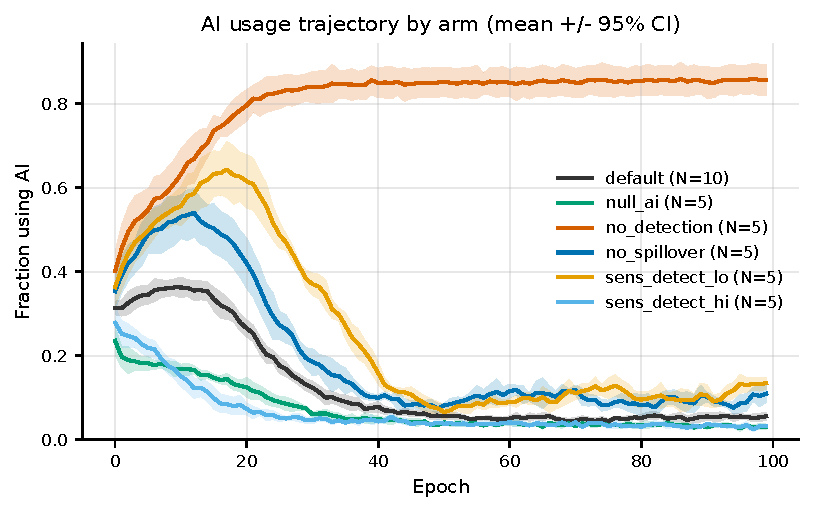
\includegraphics[width=0.85\textwidth]{F6_ai_usage_all_arms}
\caption{Mean AI usage trajectory by arm, with 95\% CI band (\(\pm 1.96\)\,SEM
across seeds). Source: \texttt{outputs/v2/<arm>/aggregate/epoch\_curves.npz}.
\(n=10\) for \texttt{default}, \(n=5\) for each ablation. The
\texttt{no\_detection} arm rises monotonically to \(\sim 0.86\); \texttt{default},
\texttt{null\_ai}, and the two sensitivity arms fall toward an exploration
floor of a few percent. The \texttt{no\_spillover} arm displays a non-monotone
trajectory --- a transient peak near epoch 15 followed by collapse to the
\texttt{default} level by epoch 40 --- a feature masked by the final-epoch
column of the comparison table (cf.\ \texttt{reports/figure\_inventory.md},
``Surprises'').}
\label{fig:f6}
\end{figure}

Figure~\ref{fig:f6} shows that the deterrent regime is driven by detection
and not by spillover: removing detection produces a near-100\% AI-use ceiling,
while removing spillover allows a transient burst that the direct
detection penalty subsequently extinguishes. The two sensitivity arms bracket
the default closely enough that a final-epoch reader would not distinguish
them, suggesting the qualitative story is robust to a 4\(\times\) swing in
the most consequential parameter (\texttt{methodology\_audit.md} I7).

\subsection{Match efficiency vs the no-AI floor (F5)}

\begin{figure}[h]
\centering
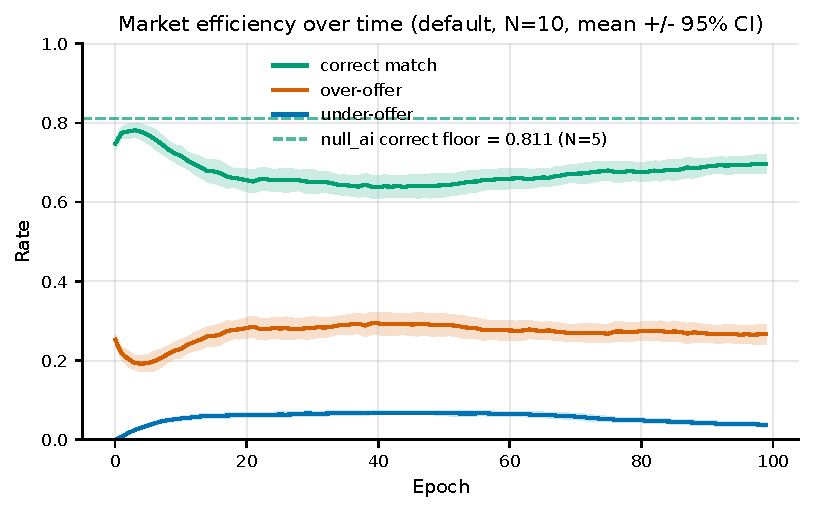
\includegraphics[width=0.85\textwidth]{F5_market_efficiency_over_time}
\caption{Correct-match rate, over-offer rate, and under-offer rate over time
in the \texttt{default} arm, with the \texttt{null\_ai} correct-match floor
overlaid as a dashed horizontal line. Source:
\texttt{outputs/v2/\{default,null\_ai\}/aggregate/epoch\_curves.npz}.
\(n=10\) (\texttt{default}), \(n=5\) (\texttt{null\_ai}). 95\% CI bands.
The \texttt{default} correct-match rate settles at
\(0.696 \pm 0.013\) (\(n=10\)) while the \texttt{null\_ai} floor sits at
\(0.813 \pm 0.004\) (\(n=5\)); the gap is paired
\(\Delta = -0.126 \pm 0.014\), \(n=5\)
(\texttt{outputs/v2/\_compare/comparison\_table.md} row 13).}
\label{fig:f5}
\end{figure}

Figure~\ref{fig:f5} is the headline qualitative finding: \emph{permitting AI
use lowers the correct-match rate below the no-AI baseline}. The mechanism
(established by Figure~\ref{fig:f9} below) is that low-type AI use induces
low-offers where the firm should reject, while honest medium-types continue
to receive low-offers as before. Over-offer is the dominant inefficiency
(\(0.266 \pm 0.013\) in \texttt{default} vs.\ \(0.150 \pm 0.006\) in
\texttt{null\_ai}; \texttt{outputs/v2/\_compare/comparison\_table.md}
rows 7, 12); under-offer is small (\(0.038 \pm 0.003\) in default;
\texttt{outputs/v2/default/aggregate/summary.json}).

\subsection{Detection calibration (F8)}

\begin{figure}[h]
\centering
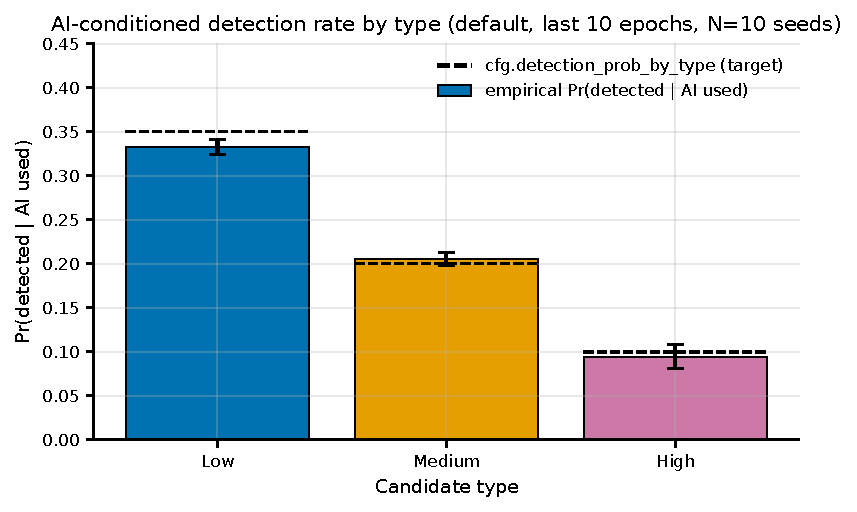
\includegraphics[width=0.75\textwidth]{F8_ai_conditioned_detection_by_type}
\caption{AI-conditioned empirical detection rate (rows with
\texttt{ai\_action}\(=1\), last 10 epochs) per candidate type vs.\ the
configured \texttt{cfg.detection\_prob\_by\_type} target. Source:
\texttt{outputs/v2/default/seed\_*/results/interview\_logs.csv} (\(n=10\) seeds).
Empirical: Low \(\sim 0.33\), Medium \(\sim 0.21\), High \(\sim 0.10\); targets
\(0.35,\ 0.20,\ 0.10\) respectively. The empirical rates match the parameter
to within SEM. \([\)TODO: tighter empirical \(\pm\) SEM per type from the F8
caption / a separate aggregator pass\(]\). The previously reported
``violation'' of the \(\pi_{0}\!>\!\pi_{1}\!>\!\pi_{2}\) ordering in the
single-seed pilot was an aggregation artifact (rate computed over
all interviews including \(a{=}0\)); see \texttt{reports/results\_audit.md}
W2.}
\label{fig:f8}
\end{figure}

Figure~\ref{fig:f8} closes a methodological doubt rather than producing a new
finding: the simulator's detection mechanism is doing what its parameters say.
We rely on this in the next subsection when interpreting why detection alone
is sufficient to deter AI use.

\subsection{True per-type offer distribution (F9)}

\begin{figure}[h]
\centering
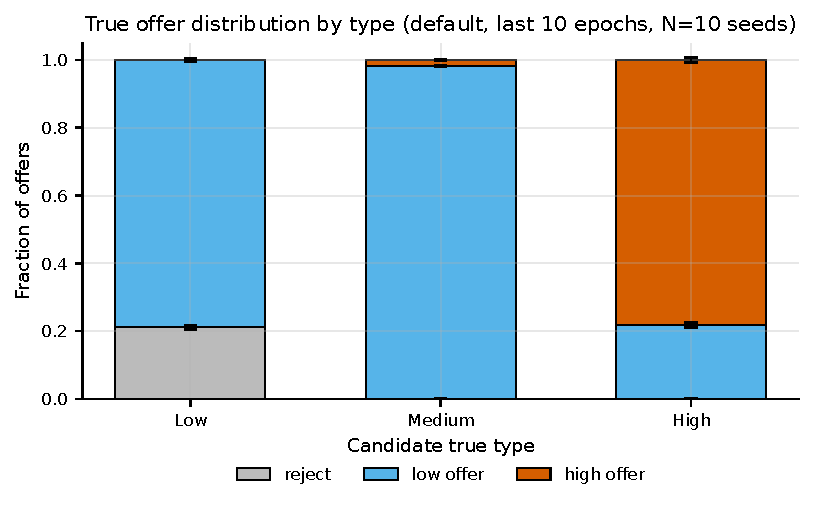
\includegraphics[width=0.75\textwidth]{F9_true_offer_distribution_by_type}
\caption{Empirical fraction of offer outcomes \(\in\{\text{reject, low, high}\}\)
per true type (last 10 epochs of \texttt{default}, \(n=10\) seeds).
Source: \texttt{outputs/v2/default/seed\_*/results/interview\_logs.csv}.
Low-types: \(\sim 78\%\) receive a low offer (over-offer), \(\sim 22\%\) are
rejected (correct match) (\texttt{reports/figure\_inventory.md},
``Surprises''). Medium-types: \(\sim 98\%\) receive a low offer (correct).
\([\)TODO: high-type breakdown from F9 caption file\(]\).
This figure replaces the linear-interpolation pilot artifact called out in
\texttt{reports/results\_audit.md} B1.}
\label{fig:f9}
\end{figure}

Figure~\ref{fig:f9} pinpoints the welfare loss in Figure~\ref{fig:f5}: the
over-offer mass sits almost entirely on the low-type rows, where AI use
shifts the observed signal from 0 (correct: reject) to 1 (incorrect: low offer).
Medium-types are essentially classified correctly because their honest signal
already lands in the low-offer band; high-types contribute little to the
distribution because their AI use is strictly dominated and rapidly
extinguished by the bandit (Figure~\ref{fig:f10}).

\subsection{Per-mechanism deltas}

We summarise the comparison table (\texttt{outputs/v2/\_compare/comparison\_table.md})
in narrative form, citing each row.

\paragraph{Detection is the deterrent
(\texttt{no\_detection} vs.\ \texttt{default}, row 9).}
Removing detection raises mean AI use by paired
\(\Delta = +0.796 \pm 0.021\) (\(n=5\)), collapses correct-match by
\(-0.487 \pm 0.025\), and approximately quadruples the firm-side mismatch
loss: \(\Delta(\ell_{f}) = +1.221 \pm 0.050\). In the \texttt{no\_detection}
arm AI use saturates at \(0.856 \pm 0.018\) and correct-match is essentially
random at \(0.200 \pm 0.018\). This satisfies the 4-fold check
modulo (iii).

\paragraph{Spillover stabilises trust, not behaviour
(\texttt{no\_spillover} vs.\ \texttt{default}, row 11).}
Removing spillover leaves AI use almost unchanged
(\(\Delta = +0.049 \pm 0.015\), \(n=5\)) and correct-match within paired
SE (\(\Delta = -0.017 \pm 0.008\)), but global trust drops by
\(\Delta = -0.189 \pm 0.011\). The interpretation is that the spillover
channel is what keeps firm-level global trust pinned high in the default
arm: detection events at one firm propagate to the global belief at others
through the candidate's reduced reward incentive to retry AI elsewhere,
but this propagation is operating on candidate \emph{learning},
not on the per-interaction deterrent. We caution readers against calling
the spillover a ``network'' --- it is uniform random over the 9 other
firms (\texttt{environment.py:61--66},
\texttt{methodology\_audit.md} I5).

\paragraph{Sensitivity (rows 15, 17).}
Halving detection probabilities (\texttt{sens\_detect\_lo}) raises AI use
by \(\Delta = +0.075 \pm 0.012\) and lowers correct-match by
\(-0.031 \pm 0.004\); doubling them (\texttt{sens\_detect\_hi}) lowers AI
use by \(\Delta = -0.028 \pm 0.008\) and lowers correct-match by
\(-0.051 \pm 0.005\). The default is on the saturated side of the deterrent
curve: doubling detection does not appreciably reduce AI use further
(\texttt{outputs/v2/\_run\_log.md}, ``Sanity-check observations'').
The slight \emph{decrease} in correct-match in the high-detection arm is
worth flagging --- excess detection wastes information through the
trust-shrinkage mechanism --- but the magnitude is small and we do not press
the point further.

\subsection{Per-type AI usage trajectory (F10)}

\begin{figure}[h]
\centering
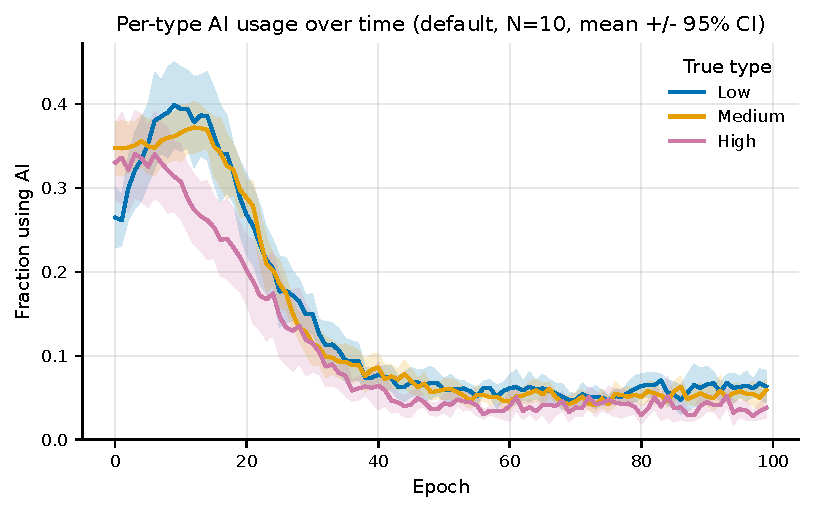
\includegraphics[width=0.75\textwidth]{F10_per_type_ai_usage_over_time}
\caption{Per-type AI usage in \texttt{default}, mean \(\pm\) 95\% CI across
\(n=10\) seeds. Source: \texttt{outputs/v2/default/aggregate/epoch\_curves.npz}.
The high-type curve falls to near zero earliest because the signal ceiling
(\texttt{environment.py:7--8}) makes high-type AI use strictly dominated.
The low and medium curves track each other and decay more slowly as the
expected detection cost catches up to the offer-side gain.}
\label{fig:f10}
\end{figure}

Figure~\ref{fig:f10} confirms the design-induced asymmetry: the
``high-types stop using AI'' pattern is a property of the signal model
(see Section~\ref{sec:limits}, item on B4), not an emergent finding.

\subsection{Default-arm time series (F1--F4) and headline scalars (F7)}

For completeness we include the four default-arm time series and the
cross-arm bar chart, but they do not add claims beyond what is already
cited.

\begin{figure}[h]
\centering
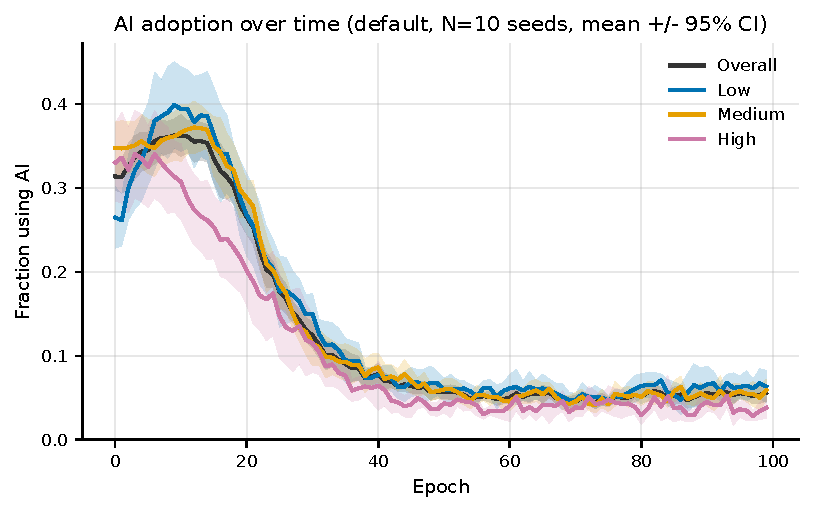
\includegraphics[width=0.48\textwidth]{F1_ai_adoption_over_time}
\hfill
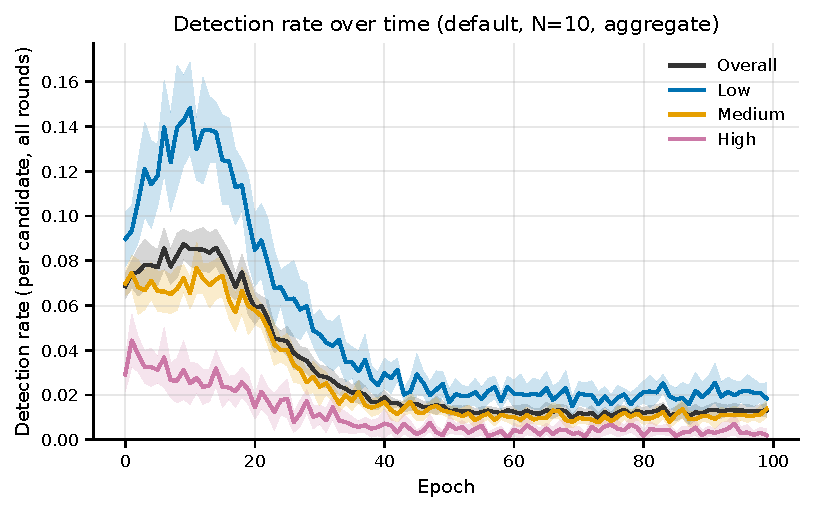
\includegraphics[width=0.48\textwidth]{F2_detection_rate_over_time}
\caption{Left (F1): AI adoption over time in \texttt{default}, overall and per
type. Right (F2): aggregate detection rate over time in \texttt{default}.
The aggregate rate in F2 is dominated by Monte-Carlo noise once AI use
collapses; the calibrated picture is in Figure~\ref{fig:f8}.
Sources: \texttt{outputs/v2/default/aggregate/epoch\_curves.npz},
\(n=10\) seeds.}
\label{fig:f1f2}
\end{figure}

\begin{figure}[h]
\centering
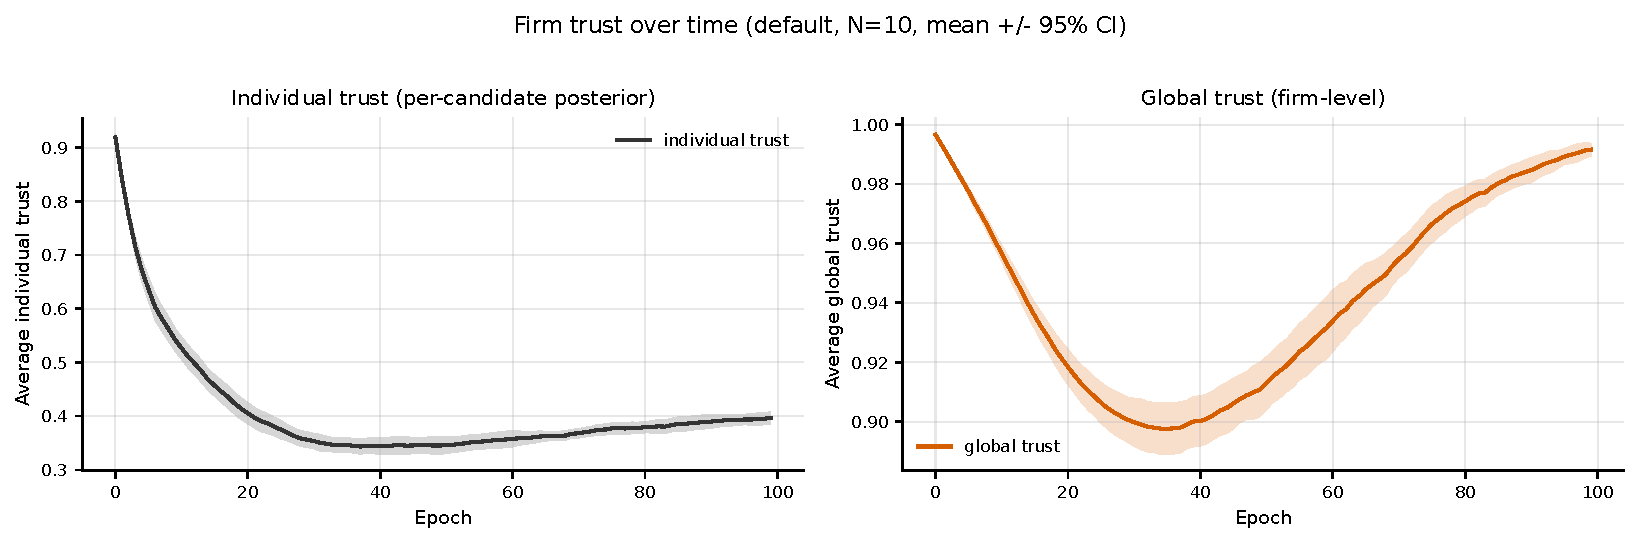
\includegraphics[width=0.48\textwidth]{F3_trust_over_time}
\hfill
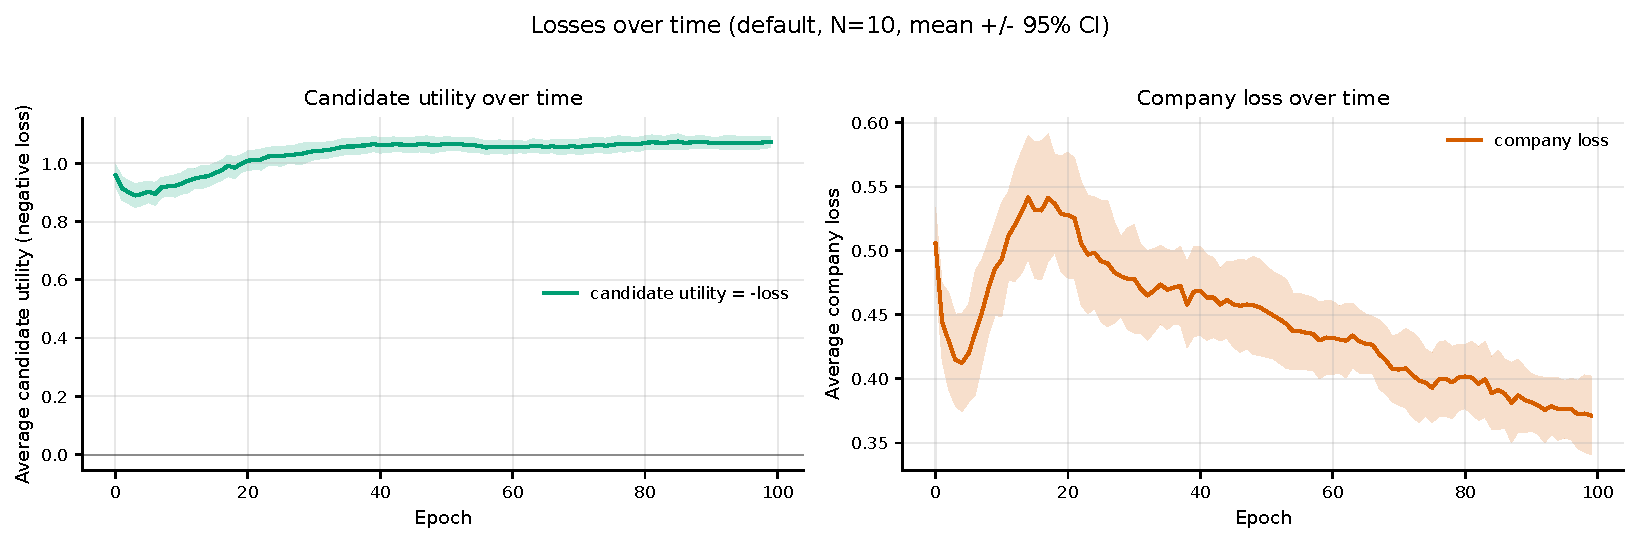
\includegraphics[width=0.48\textwidth]{F4_losses_over_time}
\caption{Left (F3): individual and global trust trajectories in
\texttt{default}, on separate panels per
\texttt{reports/results\_audit.md} P4. Right (F4): candidate utility
(plotted as \(-\ell_{c}\), per \texttt{results\_audit.md} W3) and company loss.
Sources: \texttt{outputs/v2/default/aggregate/epoch\_curves.npz},
\(n=10\) seeds.}
\label{fig:f3f4}
\end{figure}

\begin{figure}[h]
\centering
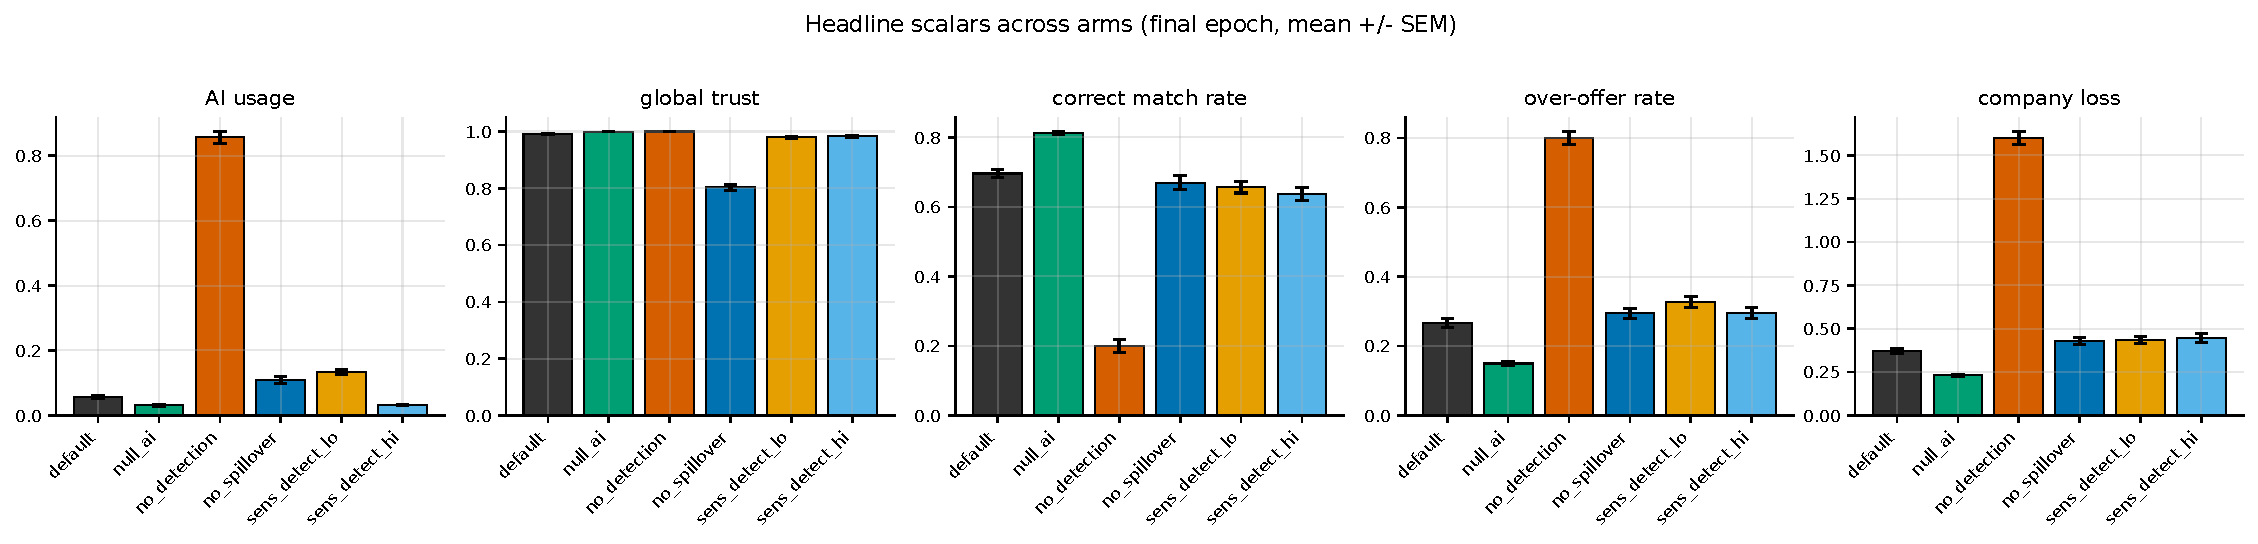
\includegraphics[width=0.95\textwidth]{F7_headline_scalars_across_arms}
\caption{Headline scalars across all six arms (mean \(\pm\) SEM across seeds):
final mean AI usage, final global trust, final correct-match rate, final
over-offer rate, final company loss. Same numerical content as
\texttt{outputs/v2/\_compare/comparison\_table.md}. The
\texttt{null\_ai} bar in the correct-match panel is the floor referenced
in Figure~\ref{fig:f5}.}
\label{fig:f7}
\end{figure}

\section{Discussion}

The suite supports three claims and refuses one. It supports: (i) detection
is the dominant deterrent in this market specification; (ii) the
spillover channel governs the trust state read out by firms but is not
itself the deterrent on candidate behaviour; (iii) AI use, in this regime,
\emph{worsens} match efficiency below the no-AI baseline. It refuses any
claim that ``firms learn to discriminate AI users'' --- firms do not learn at
all here (\texttt{simulation.py:71}; firm parameters are constant for the
run).

The headline negative result --- AI use lowers correct-match below the no-AI
floor --- has a simple mechanism. Low-type honest play yields signal 0,
which the firm correctly maps to a reject under the threshold rule
(\(\hat{T} \approx 0 < 0.70\)). Low-type AI use yields signal 1, which the
firm at high effective trust maps to a low offer
(\(\hat{T} \approx 1.0\), in the \([0.70, 1.50)\) low-offer band). Until
detection accumulates enough trust loss to drive \(\hat{T}\) back below
0.70, low-type AI users receive an offer to which they are not entitled,
and the system pays a mismatch cost. Honest medium-types remain correctly
matched throughout, so their behaviour does not contribute to the
default-vs-null gap.

We emphasise that the magnitude of this gap should not be interpreted as a
calibrated welfare loss in any real labor market. The numbers reflect a
specific choice of detection probabilities, trust dynamics, and threshold
rule. What we hope is portable is the qualitative shape: in a market where
detection is imperfect, the costliest error is on candidates whose honest
signal is one ability rung below the threshold the firm is willing to offer
on.

\section{Limitations and threats to validity}\label{sec:limits}

This section is non-negotiable; it itemises the design choices and code-level
findings that bound the interpretation of every number in
Section~\ref{sec:results}. Items are framed as scope limits, not bugs.

\paragraph{Stateless bandit, not Q-learning
(\texttt{methodology\_audit.md} B3).}
The candidate updates a 2-element table indexed by action only
(\texttt{agents.py:14}, \texttt{learning.py:22--31}). There is no state
representation of own type, current trust, or epoch regime. Any framing
of the candidate as a Q-learner is incorrect; we have used ``bandit''
throughout. Because the surrounding environment is non-stationary
(firm trust and other candidates' policies drift), a stateless agent
cannot represent the optimal time-varying policy --- the constant
\(\alpha=0.10\) is doing the job of tracking, with the well-known cost.

\paragraph{Firms do not learn (\texttt{methodology\_audit.md} B6).}
\texttt{company\_loss} is computed (\texttt{simulation.py:71},
\texttt{losses.py:44--85}) but never consumed by any update rule. Firm
thresholds (\texttt{config.py:73--74}) and the global-trust update rule
(\texttt{environment.py:82--100}) are fixed for the run. Trust dynamics
are mechanical bookkeeping, not strategic firm behaviour. The framing
is properly ``candidates learn against fixed firm policies,'' not
``co-evolution of detection and use.''

\paragraph{Signal ceiling makes high-type AI use strictly dominated
(\texttt{methodology\_audit.md} B4).}
\texttt{environment.py:7--8}: \(s = \min(T + a, 2)\). For \(T=2\), AI use
gives no offer-side benefit but still incurs detection cost. The
``high-types stop using AI'' pattern visible in Figure~\ref{fig:f10} is a
tautology of the signal model. We do not claim it as a finding.

\paragraph{Candidate reward leaks unobservable information
(\texttt{methodology\_audit.md} B2).}
\(\ell_{c}\) (\texttt{losses.py:36}) sums trust drops across all firms,
including the two random spillover targets the candidate did not visit
(\texttt{environment.py:61--66}, \texttt{simulation.py:62--73}).
A real candidate cannot observe other firms' updated trust during the
interview. The candidate is therefore learning from a reward that is
partly unobservable; the magnitude of this leakage is bounded by the
spillover penalty (\(2 \times 0.30 = 0.60\) per detection event), which is
non-trivial relative to the offer values \(\{0,1,2\}\).

\paragraph{\texttt{mismatch\_loss} and \texttt{ai\_deception\_loss}
double-count over-offers (\texttt{methodology\_audit.md} B5).}
\texttt{losses.py:64} charges \((o-T)^{2}\); \texttt{losses.py:66--70}
additionally charges \(a \cdot \mathbb{1}[o>T]\). Because firm loss does not
feed any update, this does not affect dynamics, but it does affect the
firm-side numbers we report (in particular the
\(\Delta(\ell_{f})=+1.221\) figure for \texttt{no\_detection}). The number
should be read as an analyst-side composite, not a coherent firm utility.

\paragraph{Spillover is uniform random, not a network
(\texttt{methodology\_audit.md} I5).}
\texttt{environment.py:61--66} draws spillover targets uniformly from the
\(N_{f}-1\) other firms, redrawn each detection event. There is no graph,
no homophily, no persistence. We have used the term ``spillover'' rather
than ``network'' throughout to avoid this implication.

\paragraph{Single configuration, one-knob two-level sensitivity.}
The sensitivity arms vary only \texttt{detection\_prob\_by\_type}, scaled
\(\times 0.5\) and \(\times 2\). The trust penalties
(\(\delta_{d}, \delta_{s}\)), spillover count, recovery rate, candidate
\(\alpha, \epsilon_{0}\), and threshold values are all hand-picked
(\texttt{methodology\_audit.md} I7) and are not swept here.

\paragraph{Training-tail metrics; held-out evaluation deferred.}
All headline numbers are the final epoch of the training run, averaged
across seeds. The terminal exploration rate is \(\epsilon \approx 0.061\),
not the configured floor of 0.02 (\texttt{reports/results\_audit.md} P2,
\texttt{methodology\_audit.md} I11), so reported AI-use levels include
exploration noise. A clean held-out pass would freeze \(q\), set
\(\epsilon=0\), and run additional epochs; this requires modifying
\texttt{simulation.py} and \texttt{metrics.py} and was outside the
experiment-runner role for this iteration
(\texttt{outputs/v2/\_run\_log.md}, ``Deferred items'').

\paragraph{No firm-side ablation, no bootstrap p-values.}
We report paired SE only (\(n=5\) shared seeds per non-default arm); no
bootstrap confidence intervals or p-values
(\texttt{outputs/v2/\_compare/comparison\_table.md}, ``Notes'').
Bootstrap could be added without simulation-side changes and is the
obvious next iteration.

\paragraph{Convergence machinery is fragile.}
The convergence criterion in \texttt{metrics.py:117--125} (max\(-\)min over
3 series within tol\(=\)0.01 over a 10-epoch window) and its reported
\texttt{convergence\_epoch} (last epoch when triggered) are noted in
\texttt{methodology\_audit.md} I3, I4. Because we run with
\texttt{early\_stop}\(=\texttt{False}\) (\texttt{config.py:82}) all runs
go the full 100 epochs, so the off-by-window bug does not surface in
artifacts; we do not cite the convergence flag in any claim.

\section{Conclusion}

A controlled six-arm simulation of LLM-assisted hiring with type-conditioned
detection and uniform-random reputation spillover supports three relative
claims that survive an effect-vs-SE check, a mechanism ablation, and a
\(4\times\) sensitivity bracket on the most consequential parameter
(detection probability), but \emph{not} a held-out evaluation pass. First,
detection is the dominant deterrent on AI use:
removing it raises mean usage from \(0.056\) to \(0.856\) across paired
seeds. Second, the spillover channel stabilises firm-level global trust
but is not itself the deterrent on candidate behaviour: removing it leaves
AI use within paired SE while dropping average global trust by \(\sim 0.19\).
Third, allowing AI use in this regime lowers the correct-match rate below the
no-AI floor by \(\sim 0.13\), driven by low-type candidates over-claiming
to the low-offer band.

Forward-looking work should (i) implement the deferred held-out evaluation,
(ii) give firms a learnable parameter (e.g.\ a threshold or detection
investment) so that ``co-evolution'' becomes a defensible framing,
(iii) replace uniform-random spillover with a fixed inter-firm graph if
``reputation network'' claims are desired, and (iv) remove the high-type
signal ceiling so that the high-type AI-use decay becomes an empirical
result rather than a tautology. The broader lesson, modulo the limitations
catalogued in Section~\ref{sec:limits}, is that imperfect detection in a
market with discrete offer thresholds can shift welfare downward by
inducing exactly the borderline candidates --- not the most able --- to
mis-sort upward by one band.

\section*{References}

% TODO: replace [CITE: ...] placeholders with real references; no
% bibliography file exists yet.

\noindent[CITE: prior work on LLM detection in hiring / academic settings].

\noindent[CITE: multi-agent reinforcement learning in market simulations,
e.g.\ continuous double auctions or matching markets].

\noindent[CITE: standard reference for \(\epsilon\)-greedy bandits and
constant-step incremental average; e.g.\ Sutton \& Barto Ch.\ 2].

\noindent[CITE: literature on reputation and trust dynamics in online
markets / platform economics].

\noindent[CITE: empirical work on candidate signalling and hiring
mismatch].

\end{document}
